\documentclass[]{article}
\usepackage{amssymb,amsthm,amsmath}
\usepackage{graphicx,latexsym}
\usepackage{tikz}
\usetikzlibrary{positioning}


\begin{document}

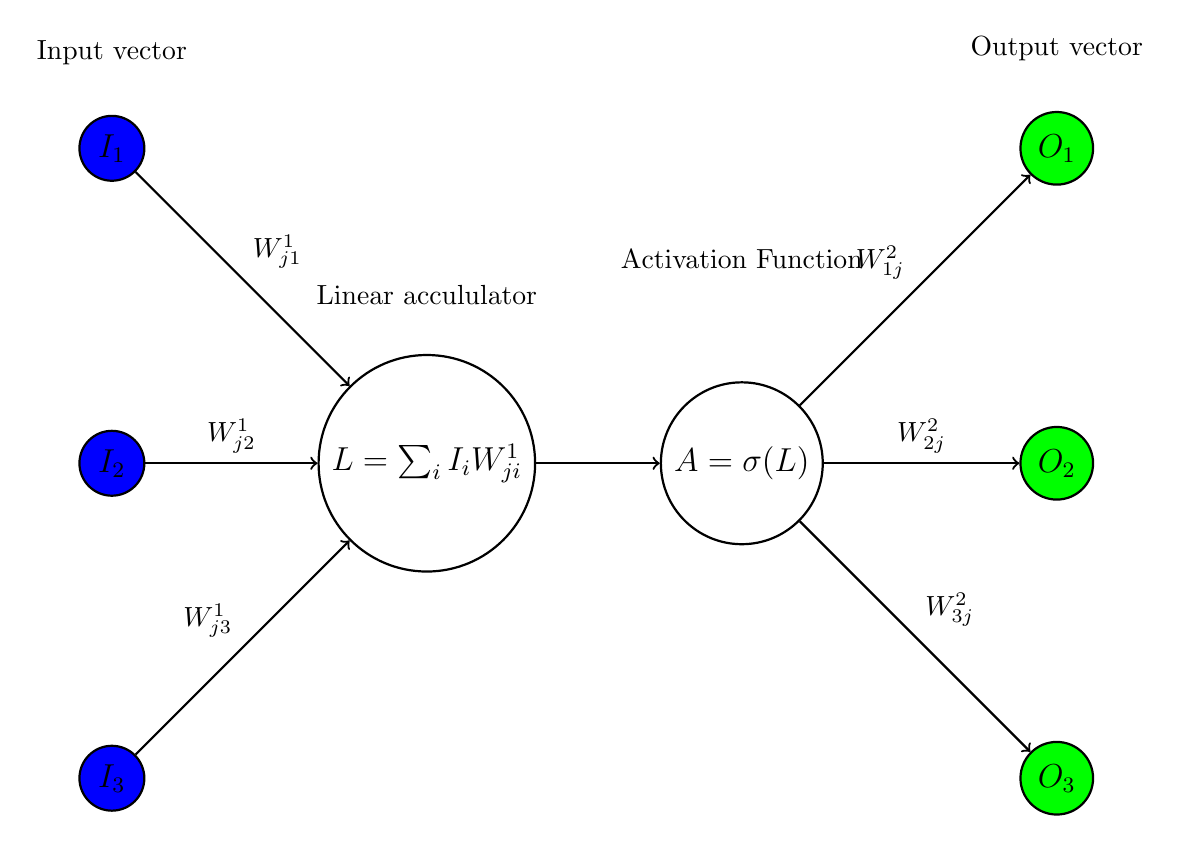
\begin{tikzpicture}[auto, node distance=4cm, every loop/.style={},
thick,main node/.style={circle,draw,font=\sffamily\large\bfseries}]

\node[main node] [fill=blue] [label={[shift={(0,0.5)}]Input vector}] (A) {$I_1$};
\node[main node] [fill=blue] (B) [below of=A] {$I_2$};
\node[main node] [fill=blue] (C) [below of=B] {$I_3$};
\node[main node] (D) [right of=B] [label={[shift={(0,0.5)}]Linear accululator}] {$L=\sum_i I_i W^1_{ji} $};
\node[main node] (P) [right of=D] [label={[shift={(0,1.3)}]Activation Function}]  {$A=\sigma(L)$};
\node[main node] [fill=green] (E) [right of=P] {$O_2$};
\node[main node] [fill=green] (F) [below of=E] {$O_3$};
\node[main node] [fill=green] (G) [above of=E] [label={[shift={(0,0.5)}]Output vector}]  {$O_1$};

\path[every node/.style={font=\sffamily\normalsize}]
(A) [->] edge node [] {$W^1_{j1}$} (D)
(B) [->] edge node [] {$W^1_{j2}$} (D)
(C) [->] edge node [] {$W^1_{j3}$} (D)
(D) [->] edge node [] {$ $} (P)
(P) [->] edge node [] {$W^2_{2j}$} (E)
(P) [->] edge node [] {$W^2_{3j}$} (F)
(P) [->] edge node [] {$W^2_{1j}$} (G);
\end{tikzpicture}

\newcommand{\cost}{c}
\newcommand{\lightred}{white!60!red}
\newcommand{\partfrac}[2]{\frac{\partial #1}{\partial #2}}
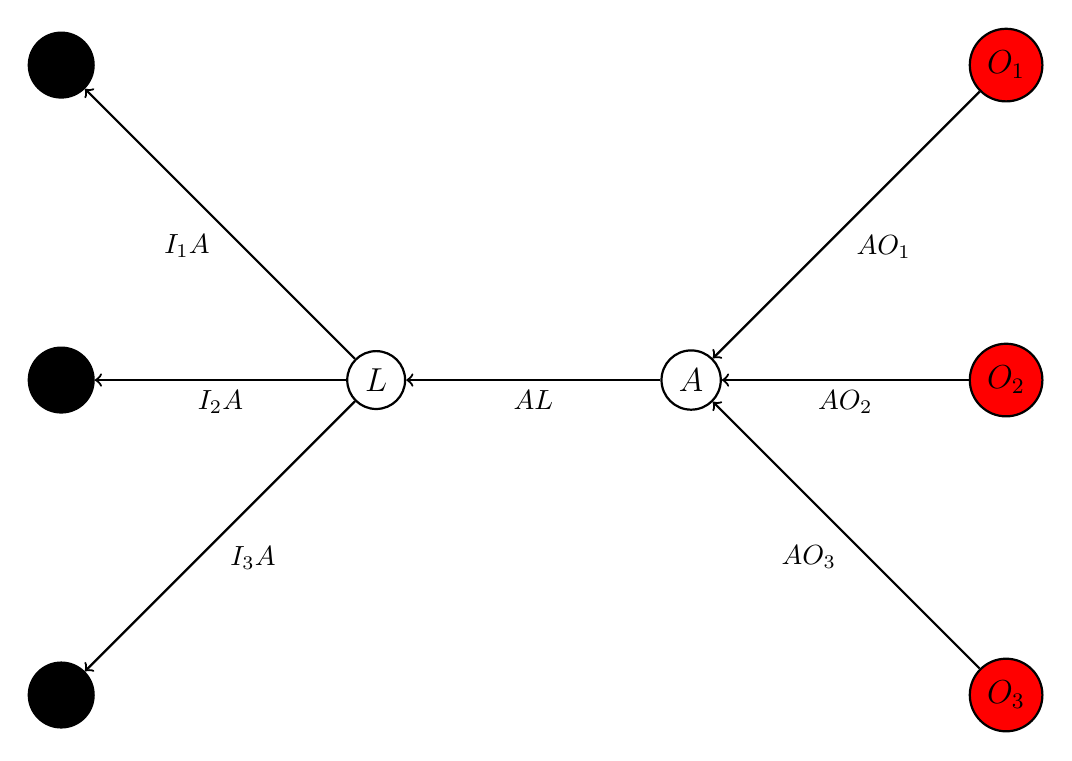
\begin{tikzpicture}[auto, node distance=4cm, every loop/.style={},
thick,main node/.style={circle,draw,font=\sffamily\large\bfseries}]

\node[main node] [fill=\lightred] (A) {$\partfrac{I_1}{\cost}$};
\node[main node] [fill=\lightred] (B) [below of=A] {$\partfrac{I_2}{\cost}$};
\node[main node] [fill=\lightred] (C) [below of=B] {$\partfrac{I_3}{\cost}$};
\node[main node] (D) [right of=B]  {$\partfrac{L}{\cost}$};
\node[main node] (P) [right of=D]   {$\partfrac{A}{\cost}$};
\node[main node] [fill=red] (E) [right of=P] {$\partfrac{O_2}{\cost}$};
\node[main node] [fill=red] (F) [below of=E] {$\partfrac{O_3}{\cost}$};
\node[main node] [fill=red] (G) [above of=E]  {$\partfrac{O_1}{\cost}$};;

\path[every node/.style={font=\sffamily\normalsize}]
(D) [->] edge node [] {$\partfrac{I_1}{A}$} (A)
(D) [->] edge node [] {$\partfrac{I_2}{A}$} (B)
(D) [->] edge node [] {$\partfrac{I_3}{A}$} (C)
(P) [->] edge node [] {$\partfrac{A}{L}$} (D)
(E) [->] edge node [] {$\partfrac{A}{O_2}$} (P)
(F) [->] edge node  {$\partfrac{A}{O_3}$} (P)
(G) [->] edge node  {$\partfrac{A}{O_1}$} (P);
\end{tikzpicture}

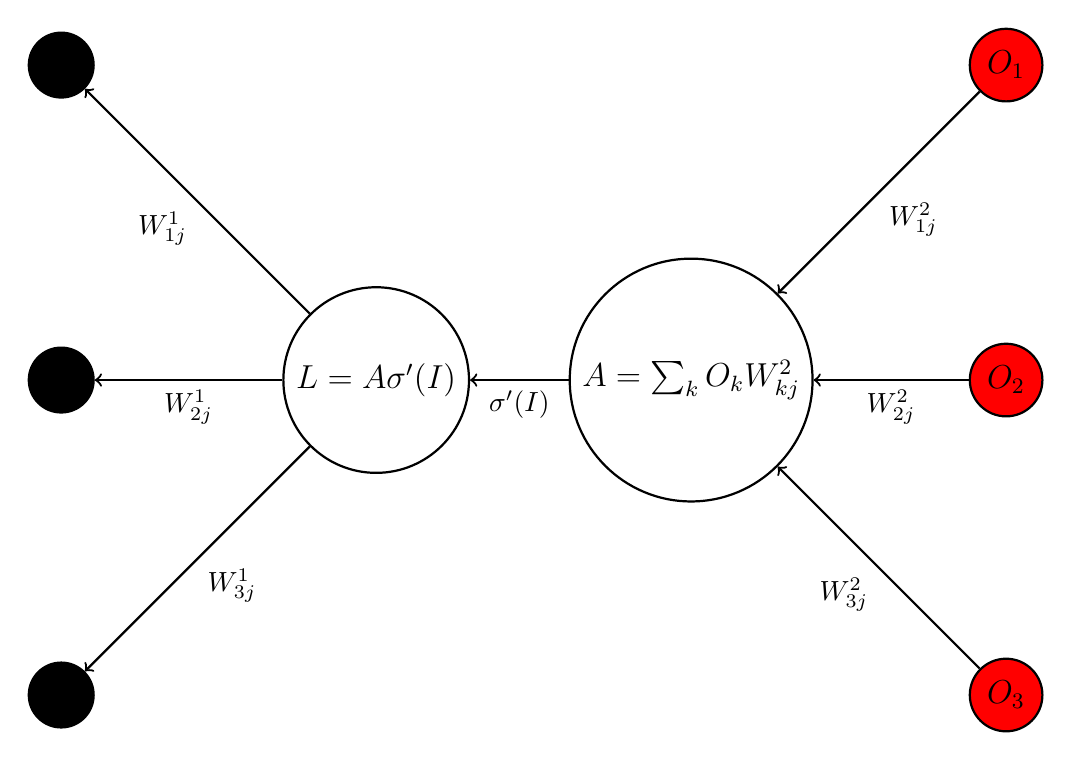
\begin{tikzpicture}[auto, node distance=4cm, every loop/.style={},
thick,main node/.style={circle,draw,font=\sffamily\large\bfseries}]

\node[main node] [fill=\lightred] (A) {$\partfrac{I_1}{\cost}$};
\node[main node] [fill=\lightred] (B) [below of=A] {$\partfrac{I_2}{\cost}$};
\node[main node] [fill=\lightred] (C) [below of=B] {$\partfrac{I_3}{\cost}$};
\node[main node] (D) [right of=B]  {$\partfrac{L}{\cost}=\partfrac{A}{\cost}\sigma^\prime(I)$};
\node[main node] (P) [right of=D]   {$\partfrac{A}{\cost}=\sum_k \partfrac{O_k}{\cost} W^2_{kj}$};
\node[main node] [fill=red] (E) [right of=P] {$\partfrac{O_2}{\cost}$};
\node[main node] [fill=red] (F) [below of=E] {$\partfrac{O_3}{\cost}$};
\node[main node] [fill=red] (G) [above of=E]  {$\partfrac{O_1}{\cost}$};;

\path[every node/.style={font=\sffamily\normalsize}]
(D) [->] edge node [] {$W^1_{1j}$} (A)
(D) [->] edge node [] {$W^1_{2j}$} (B)
(D) [->] edge node [] {$W^1_{3j}$} (C)
(P) [->] edge node [] {$\sigma^\prime(I)$} (D)
(E) [->] edge node [] {$W^2_{2j}$} (P)
(F) [->] edge node [] {$W^2_{3j}$} (P)
(G) [->] edge node [] {$W^2_{1j}$} (P);
\end{tikzpicture}


\end{document}